\section {Implementation and Technical Notes}

The code uses python 3.6 with sub-modules for questions. The repository adheres to the following:
\begin{itemize}
\item \textit{Numpy style} documentation for the module and exposed functions. 
\item A \textit{requirements.txt }for pip installing packages.
\item  Reproducible logs and reports.
\end{itemize}

\section {Question 1: Taxi Driver Problem}

\subsection{Part 1}

Dynamic Programming via the compact Bellman operators was used to solve this problem.

We implement $T(J)$ by the following vectorised code:
\begin{lstlisting}[numbers = none]
np.amax(np.sum(r*P+P*np.expand_dims(J.T,2),axis=1),axis=1)
\end{lstlisting}

We get past the fact that at \textit{town B } you cannot take action 3 (or our action 2) , by settting the rewards for action 2 (for B) as zero. Also note that since python indexing begins at zero, so do our numbering of states, stages and actions.

Where, $r$ is the reward matrix of shape (states, states, actions);
$P$ is the probability matrix of shape (states, states, actions);
$J$ is the set of states.

We do not assume the policy to be stationary (stage independent), however, this turns out to be the case in the optimal policy.

The results may be reproduced by running:
\begin{lstlisting}[numbers = none]
python3 q1.py --stages 10
\end{lstlisting}

\subsection{Part 2}

The optimal policy and rewards stage wise, for $N=10$:

\begin{lstlisting}[numbers = none]
Starting with end stage costs as [ 0.  0.  0.]
Values of J [ 16.   15.    4.5] at stage 9
Optimal policy is at stage 9 is {'state 0': 'action 1', 'state 1': 'action 1', 'state 2': 'action 2'}
Values of J [ 26.25     29.40625  18.28125] at stage 8
Optimal policy is at stage 8 is {'state 0': 'action 1', 'state 1': 'action 1', 'state 2': 'action 2'}
Values of J [ 38.265625    43.51367188  29.453125  ] at stage 7
Optimal policy is at stage 7 is {'state 0': 'action 1', 'state 1': 'action 1', 'state 2': 'action 2'}
Values of J [ 49.859375    57.30688477  41.44128418] at stage 6
Optimal policy is at stage 6 is {'state 0': 'action 1', 'state 1': 'action 1', 'state 2': 'action 2'}
Values of J [ 61.65032959  70.84981537  53.24645233] at stage 5
Optimal policy is at stage 5 is {'state 0': 'action 1', 'state 1': 'action 1', 'state 2': 'action 2'}
Values of J [ 73.44839096  84.17463732  65.14957047] at stage 4
Optimal policy is at stage 4 is {'state 0': 'action 1', 'state 1': 'action 1', 'state 2': 'action 2'}
Values of J [ 85.29898071  97.31518024  77.06275252] at stage 3
Optimal policy is at stage 3 is {'state 0': 'action 1', 'state 1': 'action 1', 'state 2': 'action 2'}
Values of J [  97.18086661  110.29839104   89.0057004 ] at stage 2
Optimal policy is at stage 2 is {'state 0': 'action 1', 'state 1': 'action 1', 'state 2': 'action 2'}
Values of J [ 109.09328351  123.1477526   100.96786822] at stage 1
Optimal policy is at stage 1 is {'state 0': 'action 1', 'state 1': 'action 1', 'state 2': 'action 2'}
Optimal policy is {'state 0': 'action 1', 'state 1': 'action 1', 'state 2': 'action 2'}
\end{lstlisting}

Clearly, the optimal policy is stationary and equal to:
\begin{lstlisting}[numbers = none]
Optimal policy is {'state 0': 'action 1', 'state 1': 'action 1', 'state 2': 'action 2'}
\end{lstlisting}

ie, ...,

\begin{itemize}
\item For towns A and B, Go to the nearest taxi stand and wait in line.
\item For town C, Wait for a call from the dispatcher.
\end{itemize}

For $N=20$;

\begin{lstlisting}[numbers = none]
Starting with end stage costs as [ 0.  0.  0.]
Values of J [ 16.   15.    4.5] at stage 19
Optimal policy is at stage 19 is {'state 0': 'action 1', 'state 1': 'action 1', 'state 2': 'action 2'}
Values of J [ 26.25     29.40625  18.28125] at stage 18
Optimal policy is at stage 18 is {'state 0': 'action 1', 'state 1': 'action 1', 'state 2': 'action 2'}
Values of J [ 38.265625    43.51367188  29.453125  ] at stage 17
Optimal policy is at stage 17 is {'state 0': 'action 1', 'state 1': 'action 1', 'state 2': 'action 2'}
Values of J [ 49.859375    57.30688477  41.44128418] at stage 16
Optimal policy is at stage 16 is {'state 0': 'action 1', 'state 1': 'action 1', 'state 2': 'action 2'}
Values of J [ 61.65032959  70.84981537  53.24645233] at stage 15
Optimal policy is at stage 15 is {'state 0': 'action 1', 'state 1': 'action 1', 'state 2': 'action 2'}
Values of J [ 73.44839096  84.17463732  65.14957047] at stage 14
Optimal policy is at stage 14 is {'state 0': 'action 1', 'state 1': 'action 1', 'state 2': 'action 2'}
Values of J [ 85.29898071  97.31518024  77.06275252] at stage 13
Optimal policy is at stage 13 is {'state 0': 'action 1', 'state 1': 'action 1', 'state 2': 'action 2'}
Values of J [  97.18086661  110.29839104   89.0057004 ] at stage 12
Optimal policy is at stage 12 is {'state 0': 'action 1', 'state 1': 'action 1', 'state 2': 'action 2'}
Values of J [ 109.09328351  123.1477526   100.96786822] at stage 11
Optimal policy is at stage 11 is {'state 0': 'action 1', 'state 1': 'action 1', 'state 2': 'action 2'}
Values of J [ 121.03057586  135.88310551  112.94817246] at stage 10
Optimal policy is at stage 10 is {'state 0': 'action 1', 'state 1': 'action 1', 'state 2': 'action 2'}
Values of J [ 132.98937416  148.52138909  124.94340833] at stage 9
Optimal policy is at stage 9 is {'state 0': 'action 1', 'state 1': 'action 1', 'state 2': 'action 2'}
Values of J [ 144.96639125  161.07701436  136.9515065 ] at stage 8
Optimal policy is at stage 8 is {'state 0': 'action 1', 'state 1': 'action 1', 'state 2': 'action 2'}
Values of J [ 156.95894887  173.56225617  148.9705143 ] at stage 7
Optimal policy is at stage 7 is {'state 0': 'action 1', 'state 1': 'action 1', 'state 2': 'action 2'}
Values of J [ 168.96473159  185.9875656   160.9988241 ] at stage 6
Optimal policy is at stage 6 is {'state 0': 'action 1', 'state 1': 'action 1', 'state 2': 'action 2'}
Values of J [ 180.98177784  198.36184213  173.03505106] at stage 5
Optimal policy is at stage 5 is {'state 0': 'action 1', 'state 1': 'action 1', 'state 2': 'action 2'}
Values of J [ 193.00841445  210.69266367  185.07802059] at stage 4
Optimal policy is at stage 4 is {'state 0': 'action 1', 'state 1': 'action 1', 'state 2': 'action 2'}
Values of J [ 205.04321752  222.9864829   197.12673118] at stage 3
Optimal policy is at stage 3 is {'state 0': 'action 1', 'state 1': 'action 1', 'state 2': 'action 2'}
Values of J [ 217.08497435  235.24879433  209.18033042] at stage 2
Optimal policy is at stage 2 is {'state 0': 'action 1', 'state 1': 'action 1', 'state 2': 'action 2'}
Values of J [ 229.13265238  247.48427659  221.23809236] at stage 1
Optimal policy is at stage 1 is {'state 0': 'action 1', 'state 1': 'action 1', 'state 2': 'action 2'}
Optimal policy is {'state 0': 'action 1', 'state 1': 'action 1', 'state 2': 'action 2'}
\end{lstlisting}

Again, the same policy.

Some comments on the rewards and policy:
\begin{itemize}
\item The rewards are unbounded - keep increasing - with stage. This is expected since there is no concept of termination in this problem.
\item We donot end up with action 3 for \textit{town B} - a sanity check.
\item It is non-optimal to only go to the nearest taxi stand. We shall show this for a stage shortly.
\end{itemize}

\subsection{Part 3}

No, it is not optimal to  to go to the nearest taxi stand, irrespective of the state.

\begin{Proof}
Assume this to be true. But, \\

\begin{align*}
J_1(C)=max_a E(r(C,j,a)) \\
& = max ( 2.5+0.5+0.25, 0.75+ 3 + 0.25, 3+ 1.5)\\
& = max( 3.25, 4, 4.5) 
\end{align*}
\\
Hence, this is not so.
\end{Proof}


\subsection {Code Blocks (pertinent only)}
\begin{lstlisting}
def T(J,verbose=False,stage=None):
    '''
    Bellman operator for maximising reward

    Args:
    * verbose: Print policy each time T is operated.
    * stage: Which stage to operate T at.
    '''
    if verbose and stage:
        policy=np.argmax(np.sum(r*P+P*J.T[np.newaxis,:,np.newaxis],axis=1),axis=1)
        cost=np.amax(np.sum(r*P+P*J[np.newaxis,:,np.newaxis],axis=1),axis=1)
        print(f"Policy at stage {stage} is {policy}, cost at stage {cost}")
    else:
        return np.amax(np.sum(r*P+P*J[np.newaxis,:,np.newaxis],axis=1),axis=1)

def read_optimal_policy(J_opt):
    '''
    Prints policy for a particular optimal J.

    Agrs:
    * J_opt: Optimal reward.
    '''
    actions= np.argmax(np.sum(r*P+P*J[np.newaxis,:,np.newaxis],axis=1),axis=1)
    return {f"state {state}":f"action {action}" for state,action in zip(range(3),actions)}
\end{lstlisting}
\bigskip

\section{Question 2}

We now use similar code to question 1, except, including this into a class \textit{Bellman} for further flexibility.

Modelling the grid-world:
\begin{itemize}
\item We use a 2D array, referenced by flattened indices for operating upon.
\item Indices go from $(0,0)$ to $(9,9)$. 
\item Again, $P$, $r$, and $J$ are modelled by tensors.
\item \textit{Wormholes}: Correspond to probabilities of 1 towards transition.
\item \textit{Terminal}: Collect a one time, at transit reward of $+100$. 
\end{itemize}

\subsection{Code Blocks (pertinent only)}

\begin{lstlisting}
P=np.zeros((100,100,4))

for i in range(100):
    # Up is +10
    if (i<90):
        P[i,i+10,0]=0.8
    else:
        P[i,i,0]=0.8
    if i%10<9:
        P[i,i+1,0]=0.1
    else:
        P[i,i,0]=0.1
    if i%10>0:
        P[i,i-1,0]=0.1
    else:
        P[i,i,0]=0.1

    # Down is -10 ...
    # Left is -1 ....
    # Right is +1 ...
    
# Wormholes
for i in [32,42,52,62]:
    for j in range(4):
        P[i,i+1,j]=0
        P[i,i-1,j]=0
        P[i,i+10,j]=0
        P[i,i-10,j]=0
        P[i,0,j]=1
        
        ....
# Terminal stage

P[terminal,terminal,:]=1
if (terminal%10)<9:
    P[terminal,terminal+1,:]=0
if (terminal%10)>0:
    P[terminal,terminal-1,:]=0
if (terminal<90):
    P[terminal,terminal+10,:]=0
if (terminal>9):
    P[terminal,terminal-10,:]=0

r=-1*np.ones((100,100,4))
r[:,terminal,:]=100
# Collect reward only once
r[terminal,terminal,:]=0
\end{lstlisting}

\subsection{Part 1}

We stop when the maximal absolute difference (np.max(np.abs()) of $J_i$ and $J_{i+1}$ falls below a certain $\epsilon$. For the sake of these three questions, we use $\epsilon = 1e-6$. \\

The intuition for this follows from the fact that $T$ is a contraction mapping, hence its repeated operations produce a Cauchy sequence in metric complete space. We have used to strength this fact.

\begin{figure}[h]
\begin{subfigure}
\centering
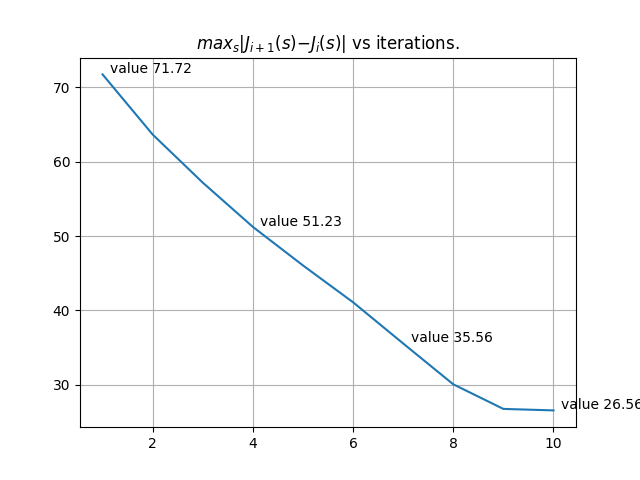
\includegraphics[angle=0,width=0.6\textwidth]{hw2/logs/t=99_N=10/convergence-till-10.png}
\caption{Convergence of $J_i$ till $N=10$ for \textbf{Terminal State (9,9)}}
\end{subfigure}

\begin{subfigure}
\centering
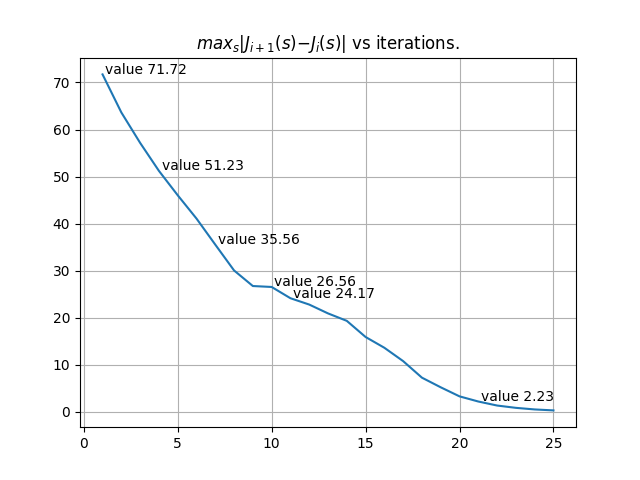
\includegraphics[angle=0,width=0.6\textwidth]{hw2/logs/t=99_N=25/convergence-till-25.png}
\caption{Convergence of $J_i$ till $N=25$ for \textbf{Terminal State (9,9)}}
\end{subfigure}

\begin{subfigure}
\centering
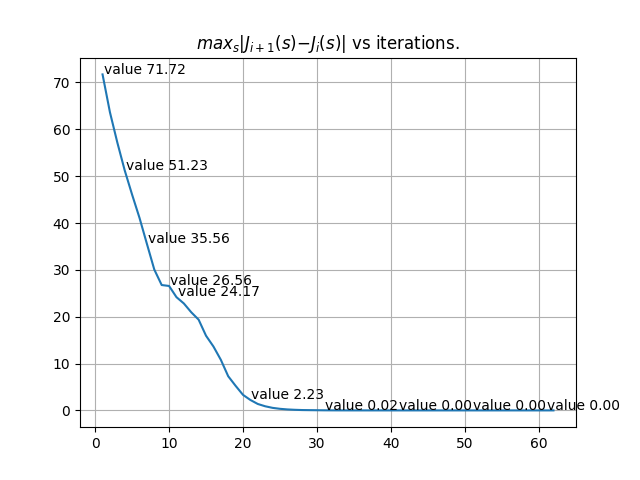
\includegraphics[angle=0,width=0.6\textwidth]{hw2/logs/t=99_N=-1/convergence-till-62.png}
\caption{Convergence of $J_i$ till absolute difference threshold for \textbf{Terminal State (9,9)}}
\end{subfigure}
\end{figure}

\begin{figure}[h]
\begin{subfigure}
\centering
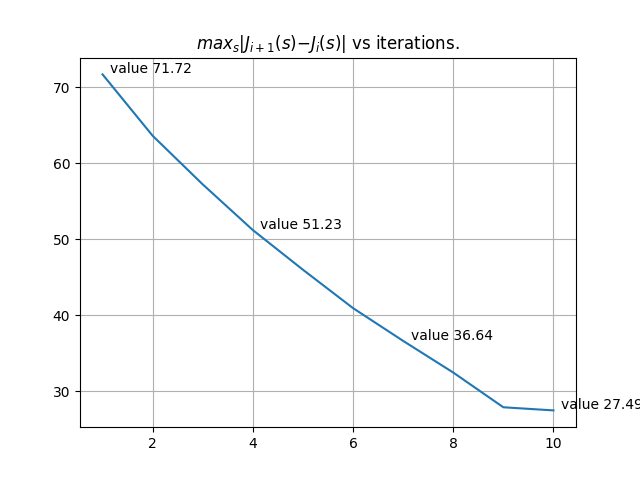
\includegraphics[angle=0,width=0.6\textwidth]{hw2/logs/t=3_N=10/convergence-till-10.png}
\caption{Convergence of $J_i$ till $N=10$ for \textbf{Terminal State (3,0)}}
\end{subfigure}

\begin{subfigure}
\centering
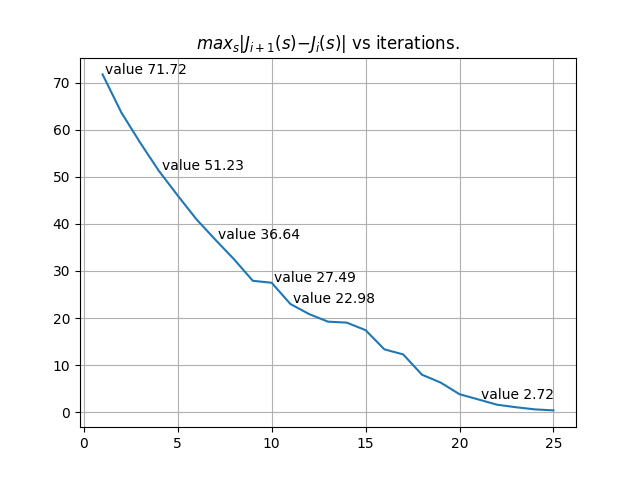
\includegraphics[angle=0,width=0.6\textwidth]{hw2/logs/t=3_N=25/convergence-till-25.png}
\caption{Convergence of $J_i$ till $N=25$ for \textbf{Terminal State (3,0)}}
\end{subfigure}

\begin{subfigure}
\centering
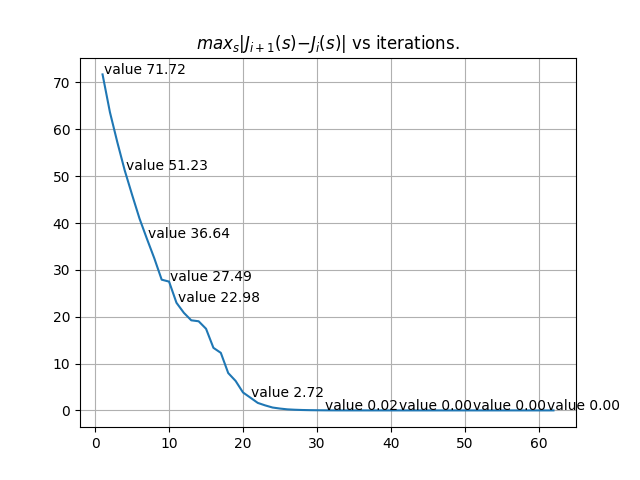
\includegraphics[angle=0,width=0.6\textwidth]{hw2/logs/t=3_N=-1/convergence-till-62.png}
\caption{Convergence of $J_i$ till absolute difference threshold for \textbf{Terminal State (3,0)}}
\end{subfigure}
\end{figure}


\subsection{Part 2 : Code Snippet}

Plots on pages 10 and 11.

\begin{lstlisting}
def plot_convergence(J_array, terminal= args.terminal, stage=0, save_path=None,supress=False):
    '''
    Plot rewards, at stages. 
    Stages are inverted here for convinience, but nonetheless holds.
    '''
    J_array=np.array(J_array)
    J_diff=np.max(np.abs(J_array[1:]-J_array[:-1]),axis=1)
    iters=np.arange(1,len(J_diff)+1)
    plt.plot(iters,J_diff)
 
    plt.grid()

    for j in range(len(J_diff)):
        if (j<10 and j%3==0) or (j%10==0):
            plt.text(j+1.15,J_diff[j]+0.15,s=f'value {J_diff[j]:.2f}')

    plt.title("$max_s |J_{i+1}(s) − J_i(s)|$ vs iterations.")

    # Save plot
    if save_path:
        plt.savefig(os.path.join(save_path,f"convergence-till-{stage}.png"))

    if not supress:
        plt.show()
    else:
        plt.close()
\end{lstlisting}

\subsection{Part 3,4}

We show the plots of $J$ and \textit{actions} as heatmaps and quiver plots respectively. \\

Plots on pages 12 to 17. \\

Comments on the plots after absolute difference convergence below a pre-determined threshold:
\begin{itemize}
\item  Wormholes are skipped wherever they lead away from the terminal state. (1 in case of (9,9), 2 in case of (3,0)).
\item  Reward to go is minimal at terminal state. (since once acquired, you terminate the game).
\item  The general policy is to either choose an apt wormhole or the direct shortest path to the terminal state.
\item  Since the probability in the intended action (Up when chosen up) is dominant, we see similar actions. If this were not the case, we could see non-obvious actions.
\item Colliding into the walls (and thereby retaining state) is discouraged, unless you happen to be at the terminal state.
\item Thus, this policy is "greedy" and does not take into account any time-variant phenomena, memory etc. Neither does solving this given grid require this.
\end{itemize}

\subsection{Code Snippet for Part 3}

\begin{lstlisting}
def quiver_actions(actions,terminal=args.terminal,stage=0, save_path=None,supress=False):
    '''
    Plot a quiver plot of the policy
    '''
    def _action_u(u):
        '''
        Horz quiver
        -1,1 if u == left or right
        0 else
        '''
        if u==2:
            return -1
        elif u==3:
            return 1
        else:
            return 0
    def _action_v(u):
        '''
        Vert quiver
        -1,1 if u == down or up
        0 else
        '''
        if u==0:
            return 1
        elif u==1:
            return -1
        else:
            return 0
    
    X=Y=np.arange(0.5,10.5,1)
    U= np.array([_action_u(a) for a in actions]).reshape((10,10))
    V= np.array([_action_v(a) for a in actions]).reshape((10,10))
    q=plt.quiver(X,Y,U,V)
    plt.quiverkey(q,X=8, Y=8, U=1,label='Quiver key, length = 1', labelpos='E')
    plt.title(f"Quiver state plot at stage {stage}")

    major_ticks = np.arange(0, 10, 1)

    # Wormholes 1
    for j in range(3,8):
        plt.scatter(2.5,j+0.5,s=225,color=colors['red'])
        plt.text(2.5, j + 0.5, 'IN1')
    # Exit 1
    plt.scatter(0.5,0.5,s=225,color=colors['maroon'])
    plt.text(0.5, 0.5, 'OUT1')

    # Wormholes 2
    plt.scatter(7.5,1.5,s=225,color=colors['grey'])
    plt.text(7.5, 1.5, 'IN2')
    plt.scatter(7.5,9.5,s=225,color=colors['lightgrey'])
    plt.text(7.5, 9.5, 'OUT2')

    # Terminal State
    a=args.terminal//10+0.5
    b=args.terminal%10+0.5
    plt.scatter(b,a,s=256,color=colors['green'])
    plt.text(b,a, 'TERMINAL')

    plt.xlim((0,10))
    plt.ylim((0,10))
    plt.xticks(major_ticks)
    plt.yticks(major_ticks)

    plt.grid(True)

    if save_path:
        plt.savefig(os.path.join(save_path,f"quiver-{stage}.png"))
    if not supress:
        plt.show()
    else:
        plt.close()
\end{lstlisting}





\begin{figure}[h]
\begin{subfigure}
\centering
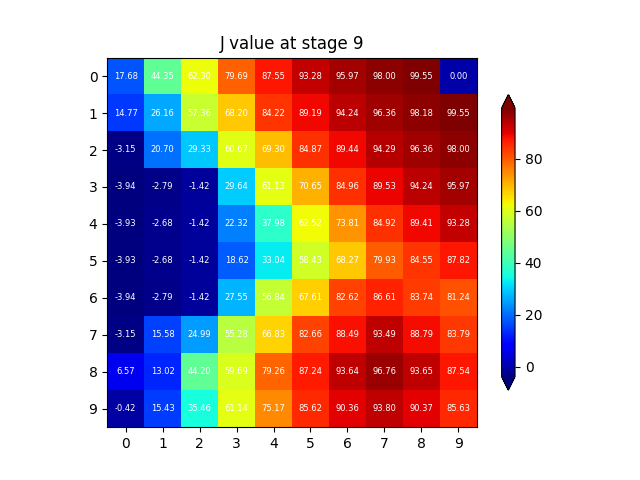
\includegraphics[angle=0,width=0.6\textwidth]{hw2/logs/t=99_N=10/J-heatmap-9.png}
\caption{Heat-map of $J_i$ till $N=10$ for \textbf{Terminal State (9,9)}}
\end{subfigure}

\begin{subfigure}
\centering
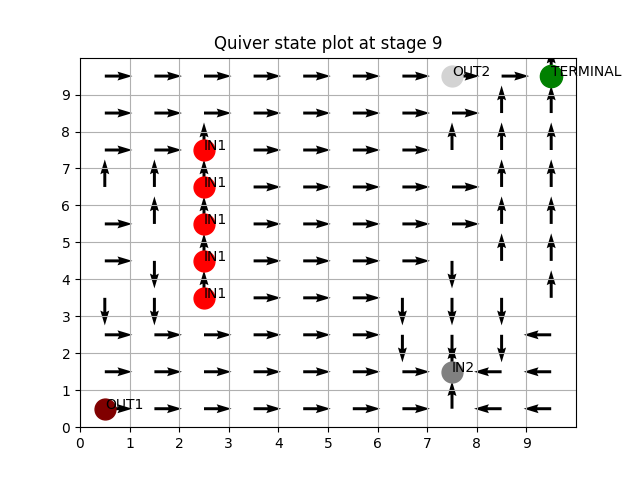
\includegraphics[angle=0,width=0.6\textwidth]{hw2/logs/t=99_N=10/quiver-9.png}
\caption{Quiver plot of $\pi$ till $N=10$ for \textbf{Terminal State (9,9)}}
\end{subfigure}
\end{figure}

\begin{figure}[h]
\begin{subfigure}
\centering
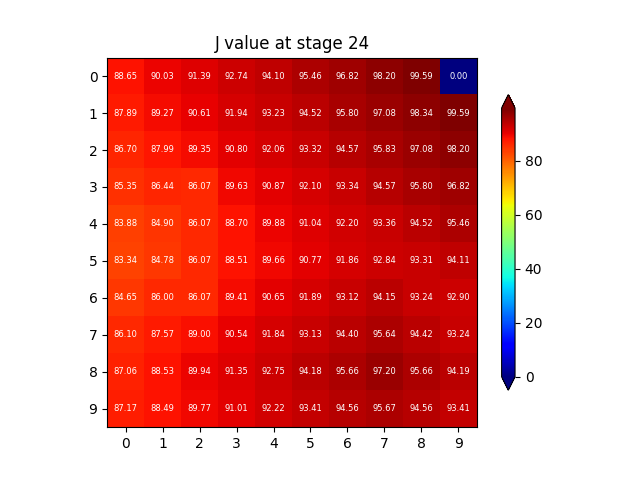
\includegraphics[angle=0,width=0.6\textwidth]{hw2/logs/t=99_N=25/J-heatmap-24.png}
\caption{Heat-map of $J_i$ till $N=25$ for \textbf{Terminal State (9,9)}}
\end{subfigure}

\begin{subfigure}
\centering
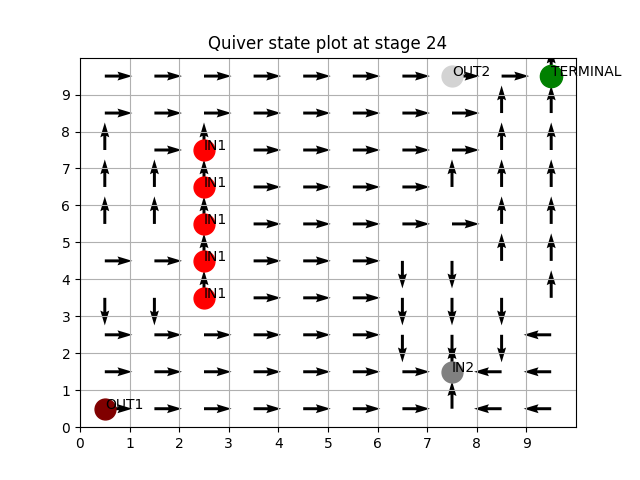
\includegraphics[angle=0,width=0.6\textwidth]{hw2/logs/t=99_N=25/quiver-24.png}
\caption{Quiver plot of $\pi$ till $N=25$ for \textbf{Terminal State (9,9)}}
\end{subfigure}
\end{figure}
\begin{figure}[h]
\begin{subfigure}
\centering
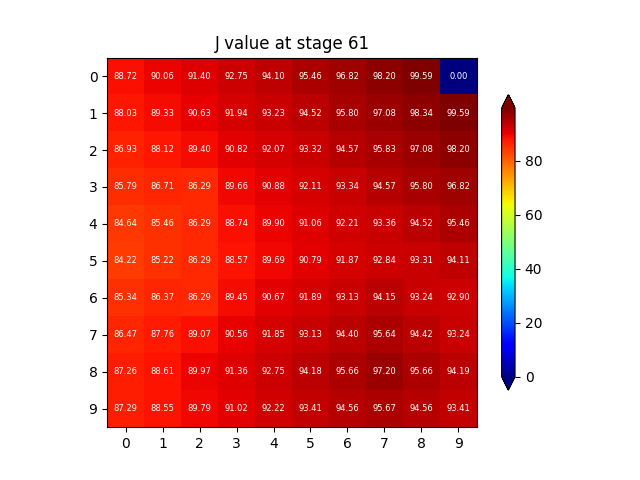
\includegraphics[angle=0,width=0.6\textwidth]{hw2/logs/t=99_N=-1/J-heatmap-61.png}
\caption{Heat-map of $J_i$ till absolute difference convergence for \textbf{Terminal State (9,9)}}
\end{subfigure}

\begin{subfigure}
\centering
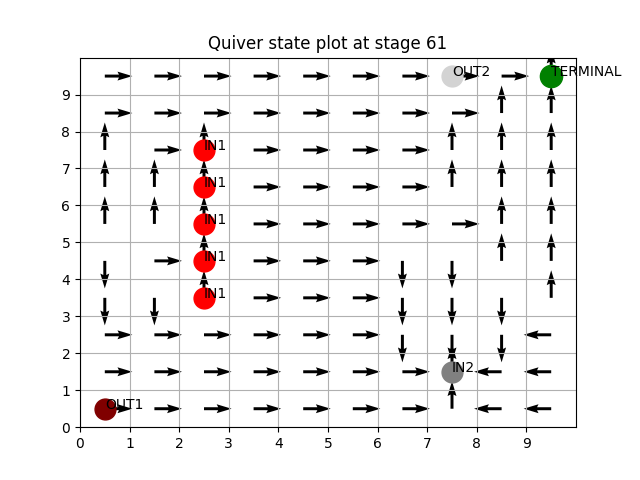
\includegraphics[angle=0,width=0.6\textwidth]{hw2/logs/t=99_N=-1/quiver-61.png}
\caption{Quiver plot of $\pi$  till absolute difference convergence for \textbf{Terminal State (9,9)}}
\end{subfigure}
\end{figure}

\begin{figure}[h]
\begin{subfigure}
\centering
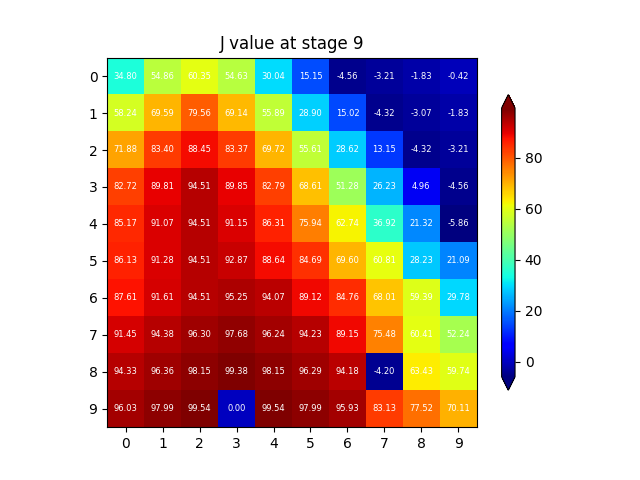
\includegraphics[angle=0,width=0.6\textwidth]{hw2/logs/t=3_N=10/J-heatmap-9.png}
\caption{Heat-map of $J_i$ till $N=10$ for \textbf{Terminal State (3,0)}}
\end{subfigure}

\begin{subfigure}
\centering
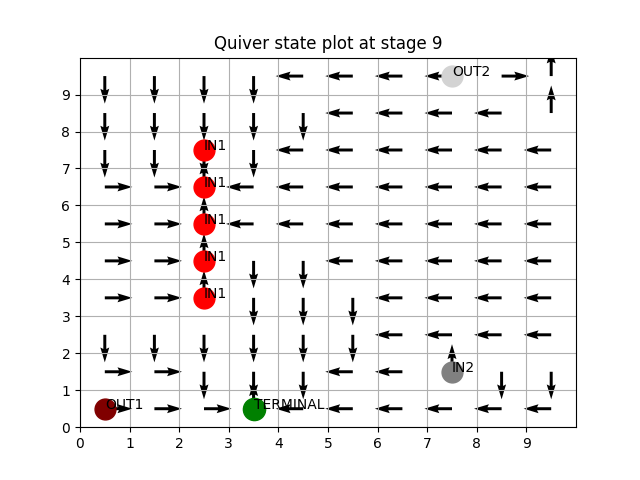
\includegraphics[angle=0,width=0.6\textwidth]{hw2/logs/t=3_N=10/quiver-9.png}
\caption{Quiver plot of $\pi$ till $N=10$ for \textbf{Terminal State (3,0)}}
\end{subfigure}
\end{figure}

\begin{figure}[h]
\begin{subfigure}
\centering
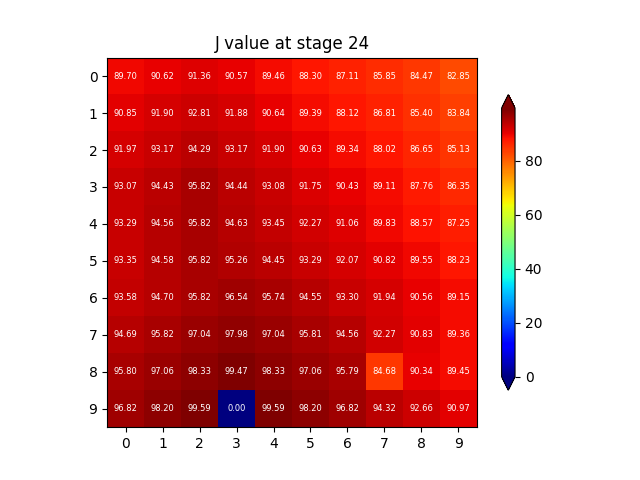
\includegraphics[angle=0,width=0.6\textwidth]{hw2/logs/t=3_N=25/J-heatmap-24.png}
\caption{Heat-map of $J_i$ till $N=25$ for \textbf{Terminal State (3,0)}}
\end{subfigure}

\begin{subfigure}
\centering
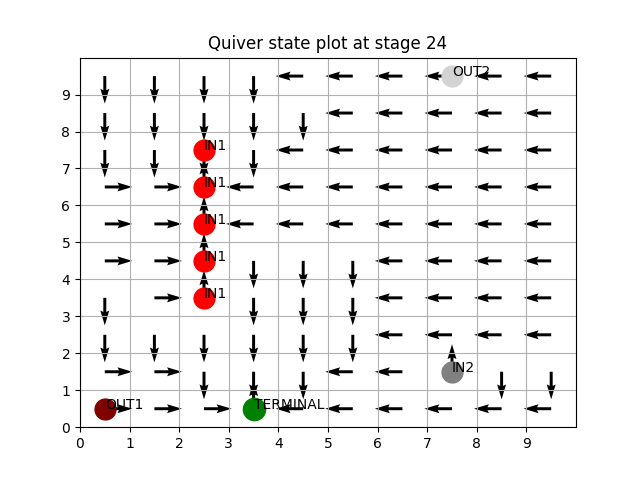
\includegraphics[angle=0,width=0.6\textwidth]{hw2/logs/t=3_N=25/quiver-24.png}
\caption{Quiver plot of $\pi$ till $N=25$ for \textbf{Terminal State (3,0)}}
\end{subfigure}
\end{figure}
\begin{figure}[h]
\begin{subfigure}
\centering
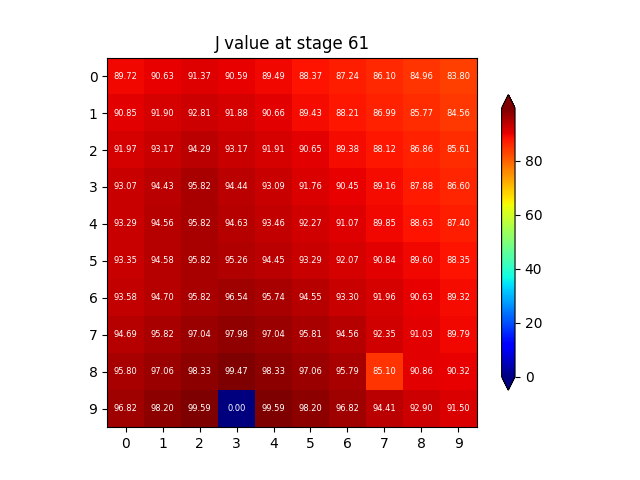
\includegraphics[angle=0,width=0.6\textwidth]{hw2/logs/t=3_N=-1/J-heatmap-61.png}
\caption{Heat-map of $J_i$ till absolute difference convergence for \textbf{Terminal State (3,0)}}
\end{subfigure}

\begin{subfigure}
\centering
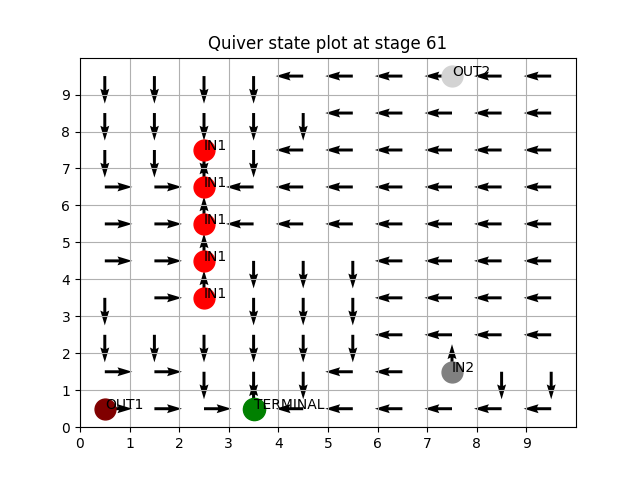
\includegraphics[angle=0,width=0.6\textwidth]{hw2/logs/t=3_N=-1/quiver-61.png}
\caption{Quiver plot of $\pi$  till absolute difference convergence for \textbf{Terminal State (3,0)}}
\end{subfigure}
\end{figure}
\section{References}
\begin{itemize}
\item Classroom lectures.
\item Bertsekas:\textit{ Dynamic Programming and Optimal Control, Vol 2, 3rd ed.}
\item Numpy, Matplotlib Dev Documentation.
\end{itemize}

